\section{Binary Star Systems}\label{sec:binary_evolution}

The evolution of a star in isolation could be summarized as:

{\it Stars contract because they are hot and lose energy through radiation (Virial Theorem), while nuclear burning cycles serve as long-lived but transitory interruptions to a star's (or at least its core's) inevitable contraction due to gravity}. 

Despite that seemingly straightforward picture, stars tend form in multiple systems (see \cref{fig:stellar_companions}). Binaries particularly, which consist of two stars that orbit around a shared center of mass and are gravitationally connected to each other, are of immense importance. By nature, they reveal more about themselves, particularly their masses and diameters, than other astronomical objects. This is especially true for eclipsing binaries \citep{prvsa2016physics}, which provide us with direct knowledge regarding spatial relations inside the source. Furthermore, close binaries are unique cosmic laboratories providing useful insights regarding different physical process. For example, gravitational wave emission is widely studied in binary mergers where both stars are compact objects \citep{cutler1994gravitational,abbott2017gw170608,abbott2019gwtc}, accretion as a power source in X-ray binaries \citep{lewin1997x,reig2011x}, while stellar interactions such as mass transfer, angular momentum exchange and tidal friction in close binaries {\it citation to be}. 


Despite the additional complexity that these stellar interactions provide to the evolution of these systems, they offer the necessary base for discussing stellar interactions in triple systems.  There are two fundamental reasons why may binaries transfer matter:

\begin{enumerate}
    \item During its evolution, one of the stars in a binary system may expand in radius (R$_{\star}$) or contract in binary separation (${\alpha}$) to the point where the companion's gravitational force can remove the outer layers of its envelope (Roche lobe overflow, RLOF).
    \item At some point in its evolution, usually during the late post-MS phases, one of the stars may release most of its mass in the form of a stellar wind; part of this material will be gravitationally trapped by the companion (stellar wind accretion). 
\end{enumerate}

This section is mainly focused on interacting binaries via RLOF, (1). 

\subsection{The Relative Orbit}

The problem of describing the motion of two point masses
under the effect of their mutual gravity, namely the famous two-body problem, has been studied extensively and a derivation of the equations of motion is out of the project's scope. For a detailed review of the two body problem, I redirect the reader to  \cite{postnov2014evolution}. Nevertheless, based on the relative orbit model, two mutually interacting bodies' equations of motion can be simplified to a single equation representing the motion of one body in a reference frame centered on the other body. The moving body therefore behaves as if its mass was
\begin{equation}\label{eq:reduced_mass}
    \mu= \frac{M_1 M_2}{M_1 + M_2}
\end{equation}
which is known as the reduced mass. As a result, the evolution of binaries can be described by the stellar masses, $M_1$ and $M_2$, the semi-major axis, $\alpha$, and the eccentricity, $e$, of the relative orbit \citep{sana2012binary,postnov2014evolution,toonen2014popcorn}. It is worth noting that the orbital separation, is linked to the eclipse's semi-major axis, although they are not equal except in the case of a circular orbit. Additionally, $\alpha$ is commonly used in the literature to define both parameters. To avoid confusion, $r_{rel}$ refers the orbital separation of the binary components and $\alpha$ to the semi-major axis of the eclipse throughout this thesis.
\begin{figure}[H]
    \centering
    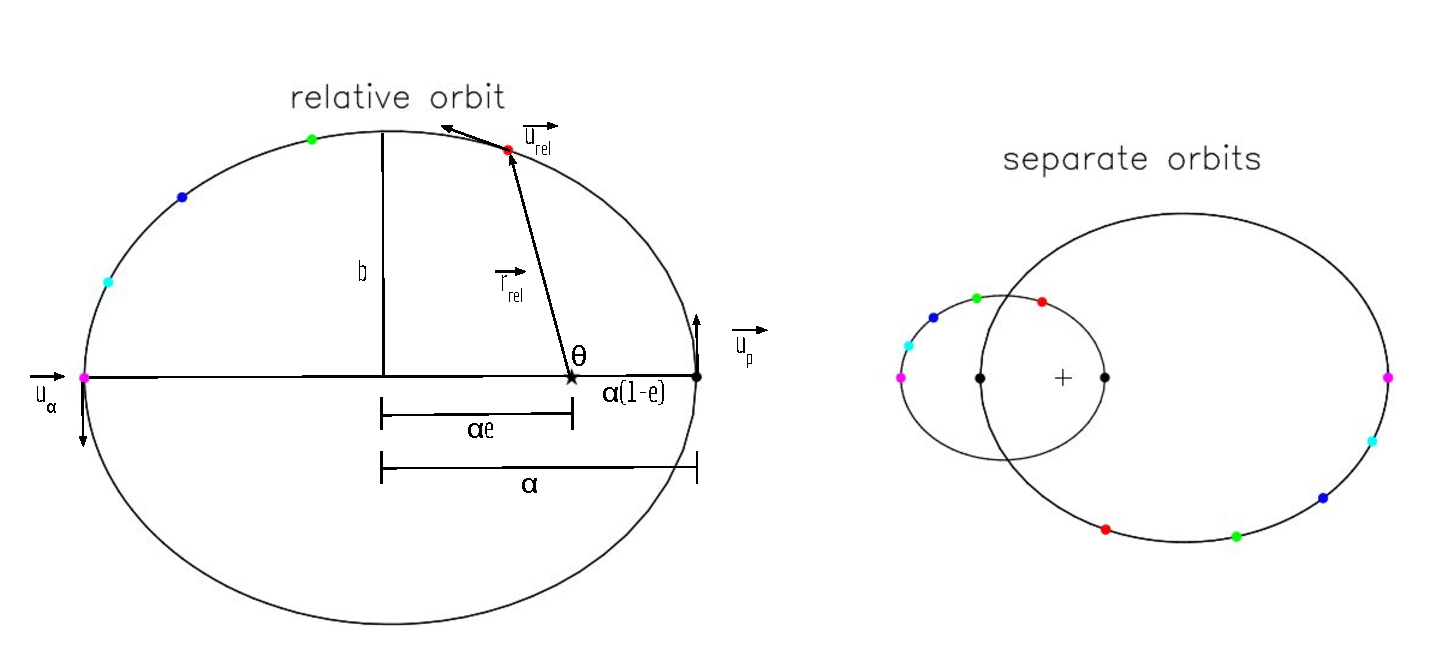
\includegraphics[width=0.9\textwidth]{Thesis/figures/relative_orbit.pdf}
    \caption{Relation between the relative orbit (left) and absolute orbits (right) of a
    binary, in this case Sirius. The black star symbol on the left figure represents the fixed star with the reference frame centered on it, while the circles represent the moving star with mass $\mu$. The absolute positions (right) are matched with the relative position of the moving body (left) via different colors.   The initial figure was taken by Frank Verbunt's lecture notes `Compact Binaries` and modified by me.}
    \label{fig:relative_orbit}
\end{figure}
The shape of the relative orbit is defined by the orbital energy and angular momentum per unit of reduced mass. For an elliptic relative orbit, specifically, the orbital energy per unit of reduced mass is
\begin{equation}\label{eq:orbital_energy}
    \epsilon = \frac{E}{\mu} = - \frac{G (M_1 + M_2)}{2\alpha}, \; \; \epsilon  < 0
\end{equation}
and the angular momentum per unit of reduced mass is
\begin{equation}\label{eq:orbital_ang_momentum}
    l = \frac{L}{\mu} = \vec{r_{rel}} \times \vec{u_{rel}} =\sqrt{G (M_1 + M_2) \alpha (1-e^2)}
\end{equation}
where $e$ is the eccentricity and $\alpha$ the semi-major axis of the eclipse, see \cref{fig:relative_orbit}. In the absence of mass loss, both $\epsilon$ and $l$ are constants of motion.

The relative position of the moving body, or the orbital separation of the binary components, see \cref{fig:relative_orbit}, is given as:
\begin{equation}\label{eq:relative_position}
    r_{rel} = \frac{\alpha (1-e^2)}{1+e \cos{\theta}}
\end{equation}
and its velocity as:
\begin{equation}\label{eq:relative_velocity}
    u_{rel}= \sqrt{G(M_1 +M_2) \left( \frac{2}{r_{rel}} - \frac{1}{\alpha}\right)}
\end{equation}

Eq. \eqref{eq:orbital_energy} shows that the orbital energy is independent of the eccentricity, $e$ and in the elliptic case is always negative.

Using Eq. \eqref{eq:relative_velocity}, the semi-major axis is given as:
\begin{equation}\label{eq:semi-major_axis}
    \alpha = \frac{G(M_1+M_2)r_{rel}}{2G(M_1+M_2) - u_{rel}^2 r_{rel}}.
\end{equation}
Additionally, using  Eq. \eqref{eq:orbital_ang_momentum} the eccentricity is given as:
\begin{equation}\label{eq:eccentricity}
    e = \sqrt{1 - \frac{|\vec{r_{rel}} \times \vec{u_{rel}}|^2}{G (M_1+M_2) \alpha}}.
\end{equation}

As a result, given the relative position and velocity of two stars, $M_1$ and $M_2$, the evolution of the binary can be describted using \cref{eq:semi-major_axis}, \cref{eq:eccentricity}, \cref{eq:orbital_ang_momentum} and \cref{eq:orbital_energy}.


\begin{comment}
For two stars of mass, $M_1$ at position $r_1$ and $M_2$ at position $r_2$, the the weighted mean position, namely the center of mass, can be defined as:
\begin{equation}\label{eq:center_of_mass}
    \vec{R_{cm}} = \frac{M_1 \vec{r_1} + M_2 \vec{r_2}}{M_1 + M_2}
\end{equation}
Furthermore, the reduced mass of the binary is defined as:
\begin{equation}
    \mu= \frac{M_1 M_2}{M_1 + M_2}
\end{equation}
\end{comment}


\subsection{Roche Lobe Overflow}

The orbital parameters of the relative orbital are critical in defining the Roche model, a valuable tool in describing binary evolution. The Roche model describes the effective gravitational potential of the binary and it is based on three assumptions:
\begin{enumerate}
    \item The gravitational fields of both stars are assumed to be those of point masses.
    \item The binary orbit is assumed to be circular, $e=0$.
    \item The rotation of the stellar components is assumed to be synchronized with the orbital motion. 
\end{enumerate}
The Roche potential's crucial equipotential surface, which passes through the inner Lagrangian point $L_1$, defines two Roche lobes that encircle each star. Hence, each Roche lobe defines the volume in which material is gravitationally bound to the respective star. The Roche lobe can be approximated with accuracy better than $1\%$ by a sphere of radius $R_L$:
\begin{equation}\label{eq:roche_lobe}
    \frac{R_{L,1}}{\alpha} = \frac{0.49q^{2/3}}{0.6q^{2/3} + \ln{1+q^{1/3}}}
\end{equation}
where $q =M_1 / M_2$ and $R_{L,2}$ will be given for $q =M_2 / M_1$. The Roche potential of a binary with $q=6.3/5.5 \approx 1.145$ and $\alpha = 1.24$ au is presented in \cref{fig:binary_equop}. The latter corresponds to the effective potential of $\xi$ Tau by replacing the inner binary masses, $M_1$ and $M_2$, with one star of mass $M = M_1 + M_2$.
\begin{figure}[H]
    \centering
    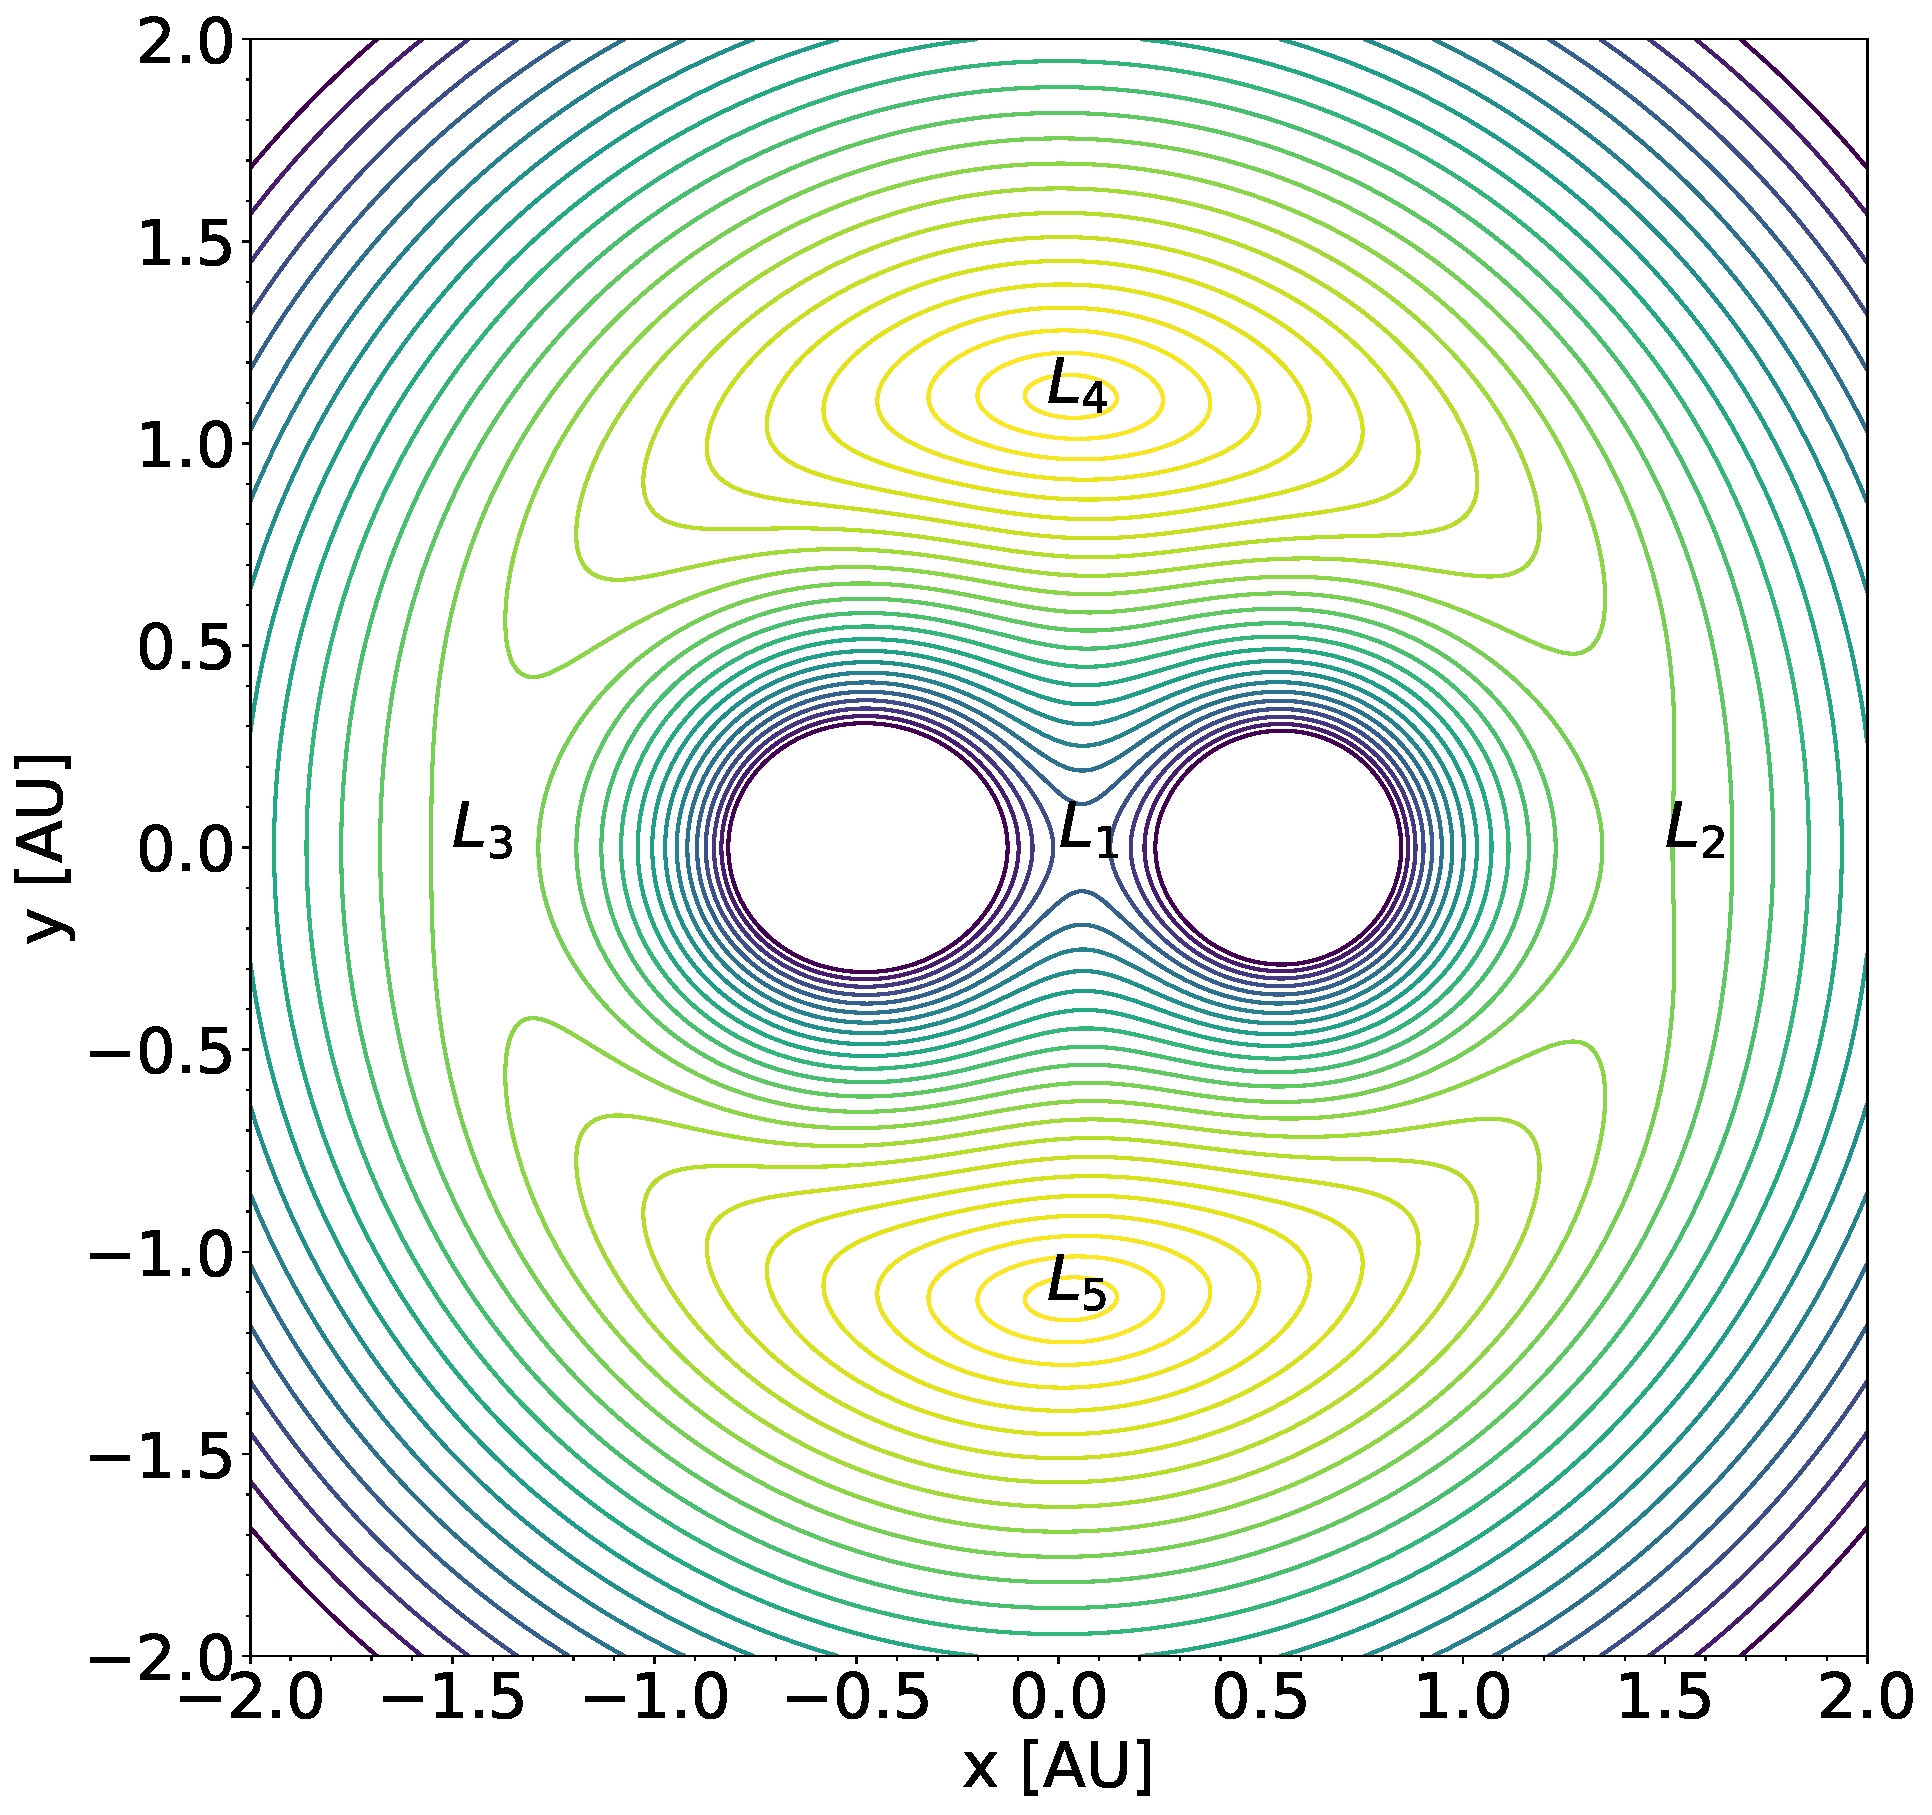
\includegraphics[width=0.9\textwidth]{Thesis/graphs/binary_equop.pdf}
    \caption{Contour plot of a binary's effective potential for $q=6.3/5.5 \approx 1.145$ and $\alpha = 1.24$ au. The five Lagrangian points are indicated as $L_1, L_2, L_3, L_4$ and $L_5$. I create the plot using the Hermite integrator which is part of AMUSE \citep{hut1995building}.}
    \label{fig:binary_equop}
\end{figure}
According to \eqref{eq:roche_lobe}, the size of the Roche lobe is determined by the mass ratio $q$ and the orbital separation of the two stars, $\alpha$. The more massive star has a larger Roche lobe, whereas stars of equal mass have equal sized Roche lobes. Furthermore, the size of the Roche lobes is proportional to the orbital separation of the stars, so as the latter changes, so do the Roche lobes.

As discussed in \cref{sec:single_star_evolution}, stars contract and expand during their evolution. Additionally, the binary separation may decrease due to the loss of orbital angular momentum from the system via stellar wind mass-loss, see \cref{sub:winds} or gravitational radiation. As a result, the physical radius of a star, $R_{\star}$, may become larger than its Roche lobe radius, $R_L$. This scenario is called Roche-lobe overflow (ROLF) and matter from the outer layers of the Roche-lobe-filling star can freely move through the first Lagrangian point $L_1$ to the companion star. 

According to \cref{sec:single_star_evolution}, intermediate-mass stars expand during MS on nuclear timescale and during RGB and AGB phases, on thermal timescale, see \cref{fig:HR_ROLF}.  Hence, three cases of mass transfer can be distinguished:
\begin{enumerate}
    \item During the MS, namely Case A
    \item During post-MS and before helium exhaustion, namely Case B
    \item After helium exhaustion, namely Case C
\end{enumerate}
Considering that mass is the most important property for a star's evolution, see \cref{sec:single_star_evolution}, ROLF can significantly alter its evolutionary outcome. Thus, in a mass-transferring binary system, both stars are expected to deviate from the evolutionary paths they would have in the absence of mass transfer. 

\subsection{Orbital Evolution During Mass Transfer}

In the case of ROLF, the transferring matter carries angular momentum causing the orbital parameters of the relative orbit to change. By differentiating Eq. \eqref{eq:orbital_ang_momentum}, a general equation for the orbital evolution can be obtained:
\begin{equation}\label{eq:orb_ang_momen_derivative}
    2\frac{\dot{J}}{J} = \frac{\dot{\alpha}}{\alpha} + 2 \frac{\dot{M_1}}{M_2} - \frac{ \dot{M_1} + \dot{M_2}}{M_1 + M_2} - \frac{2e \dot{e}}{1-e^2} 
\end{equation}
A basic assumption of \eqref{eq:orb_ang_momen_derivative} is that the angular momentum stored in the rotation of the two stars is negligible compared to the orbital angular momentum. In most circumstances, this assumption is valid, however in the case of rapidly spinning objects, such as millisecond pulsars, the angular momentum contained in the pulsar's rotation may need to be considered.  

The variable $\dot{J}$ in Eq. \eqref{eq:orb_ang_momen_derivative} represents angular momentum loss from the binary. Given the fate of the transferring mass two cases can distinguished: 
\begin{enumerate}
    \item Conservative mass transfer
    \item Non-conservative mass transfer
\end{enumerate}
Both cases are discussed in the following subsections.

\subsubsection{Conservative Mass Transfer}

In the conservative case all the mass transferred from the first star is accreted by the second and the orbital angular momentum of the binary is conserved. Thus

\begin{equation}\label{eq:mass_loss_cons}
    \dot{M_{a}} = - \dot{M_{d}}
\end{equation}
where the subscript $a$ refers to the `accretor` and $d$ to the `donor`, and
\begin{equation}\label{eq:orb_ang_mom_cons}
    \dot{J}=0
\end{equation}
Using Eq. \eqref{eq:mass_loss_cons} and \eqref{eq:orb_ang_mom_cons}, Eq. \eqref{eq:orb_ang_momen_derivative} reduces to
\begin{equation}\label{eq:orb_ang_momen_derivative_cons}
    \frac{\dot{\alpha}}{\alpha}= 2 \left( \frac{M_d}{M_a} - 1 \right) \frac{\dot{M_{d}}}{M_{d}}
\end{equation}    
A close look to Eq. \eqref{eq:orb_ang_momen_derivative_cons} reveals that the orbital separation shrinks as long as $M_d > M_a$, while it expands when $M_d < M_a$. Finally, the minimum orbital distance is given for $M_d = M_a$. 

\subsubsection{Non-Conservative Mass Transfer}

The assumption of total mass and angular momentum conservation is a helpful idealization, but it cannot be anticipated to hold in many situations. However, when mass and angular momentum loss from the binary are considered, the situation becomes considerably more difficult and ambiguous.

The mass loss can be simply parameterized as
\begin{equation}\label{eq:mass_loss_non_cons}
    \dot{M_{a}} = - \beta \dot{M_{d}}
\end{equation}
where $\beta$ is the fraction of the transferred mass that is accreted. Hence, 
\begin{equation}\label{eq:mass_loss_non_cons_2}
    \dot{M_{a}} + \dot{M_{d}} = (1 - \beta) \dot{M_{d}}
\end{equation}
will hold.